The relative composition of the diagrams shown in Figure~\ref{fig:ppTo4LG} in the signal sample was assessed in a generator level study.
The study is conducted on the four lepton channel, but the results can be generalised to the other two.
Two samples were generated at Leading Order EW ($\alpha_{\rm EW}^5 \, \alpS^0$) using \MADGRAPH.
The first is the inclusive production of four fermions and a photon, while the other constrains the intermediate vector boson state.

More precisely, the first sample simulates the process $\Pp\Pp \to 2\Pe 2\PGm \PGg$,
which in \MADGRAPH syntax corresponds to \verb|generate p p > e+ e- mu+ mu- a|.
The photon may be attached either to an initial- or final-state fermion line,
but not to a triple or quartic vertex since there are no suitable couplings in the SM for this final state.
The choice of a final state where the two lepton pairs have different flavour
excludes the interference from diagrams with the momenta of two leptons swapped.
The computed cross section is $0.075 \fbinv$.

The second sample forces the intermediate Z boson resonances $\Pp\Pp \to \PZ\PZ\PGg \to 2\Pe 2\PGm \PGg$,
using the syntax:
\begin{verbatim}
define ze = z
define zmu = z
generate p p > ze zmu a, ze > e+ e-, zmu > mu+ mu-
\end{verbatim}
In this case the photon is forced to be directly attached to an initial-state fermion line,
making this a sub-sample of the previous one.
The computed cross section is $0.027 \fbinv$.

Both samples were generated with the requirement that the leading (subleading) lepton has a transverse momentum larger than 20 (10)\GeV.
Every lepton is required to have $\pt^\Pl > 5\GeV$ and $|\eta^\Pl| < 2.5$,
while the photon must satisfy $\pt^\PGg > 20\GeV$ and $|\eta^\PGg| < 2.5$.
Additionally, the minimum separation between the photon and any of the four leptons must be $\DR(\Pl,\PGg) > 0.5$.

The distributions of the invariant mass of the same-flavour opposite-sign lepton pairs and the transverse momentum of the photon
for the first and second sample are shown in Figure~\ref{fig:genstudy}.
From these plots it appears that in a sizeable fraction of FSR events the mass of one of the
reconstructed $\Pl\Pl$ pairs is significantly lower than the \PZ peak.
It is also visible that the transverse momentum of FSR photons tends to be lower,
since the momentum of the lepton may change significantly,
and it becomes almost zero above $80\GeVc$.
However only a fraction of the events in both samples are in the tail with $\pt^\PGg > 80\GeVc$.

\begin{figure}
  \centering\hfill
  \subfigure [$m_{\Pl\Pl}$] {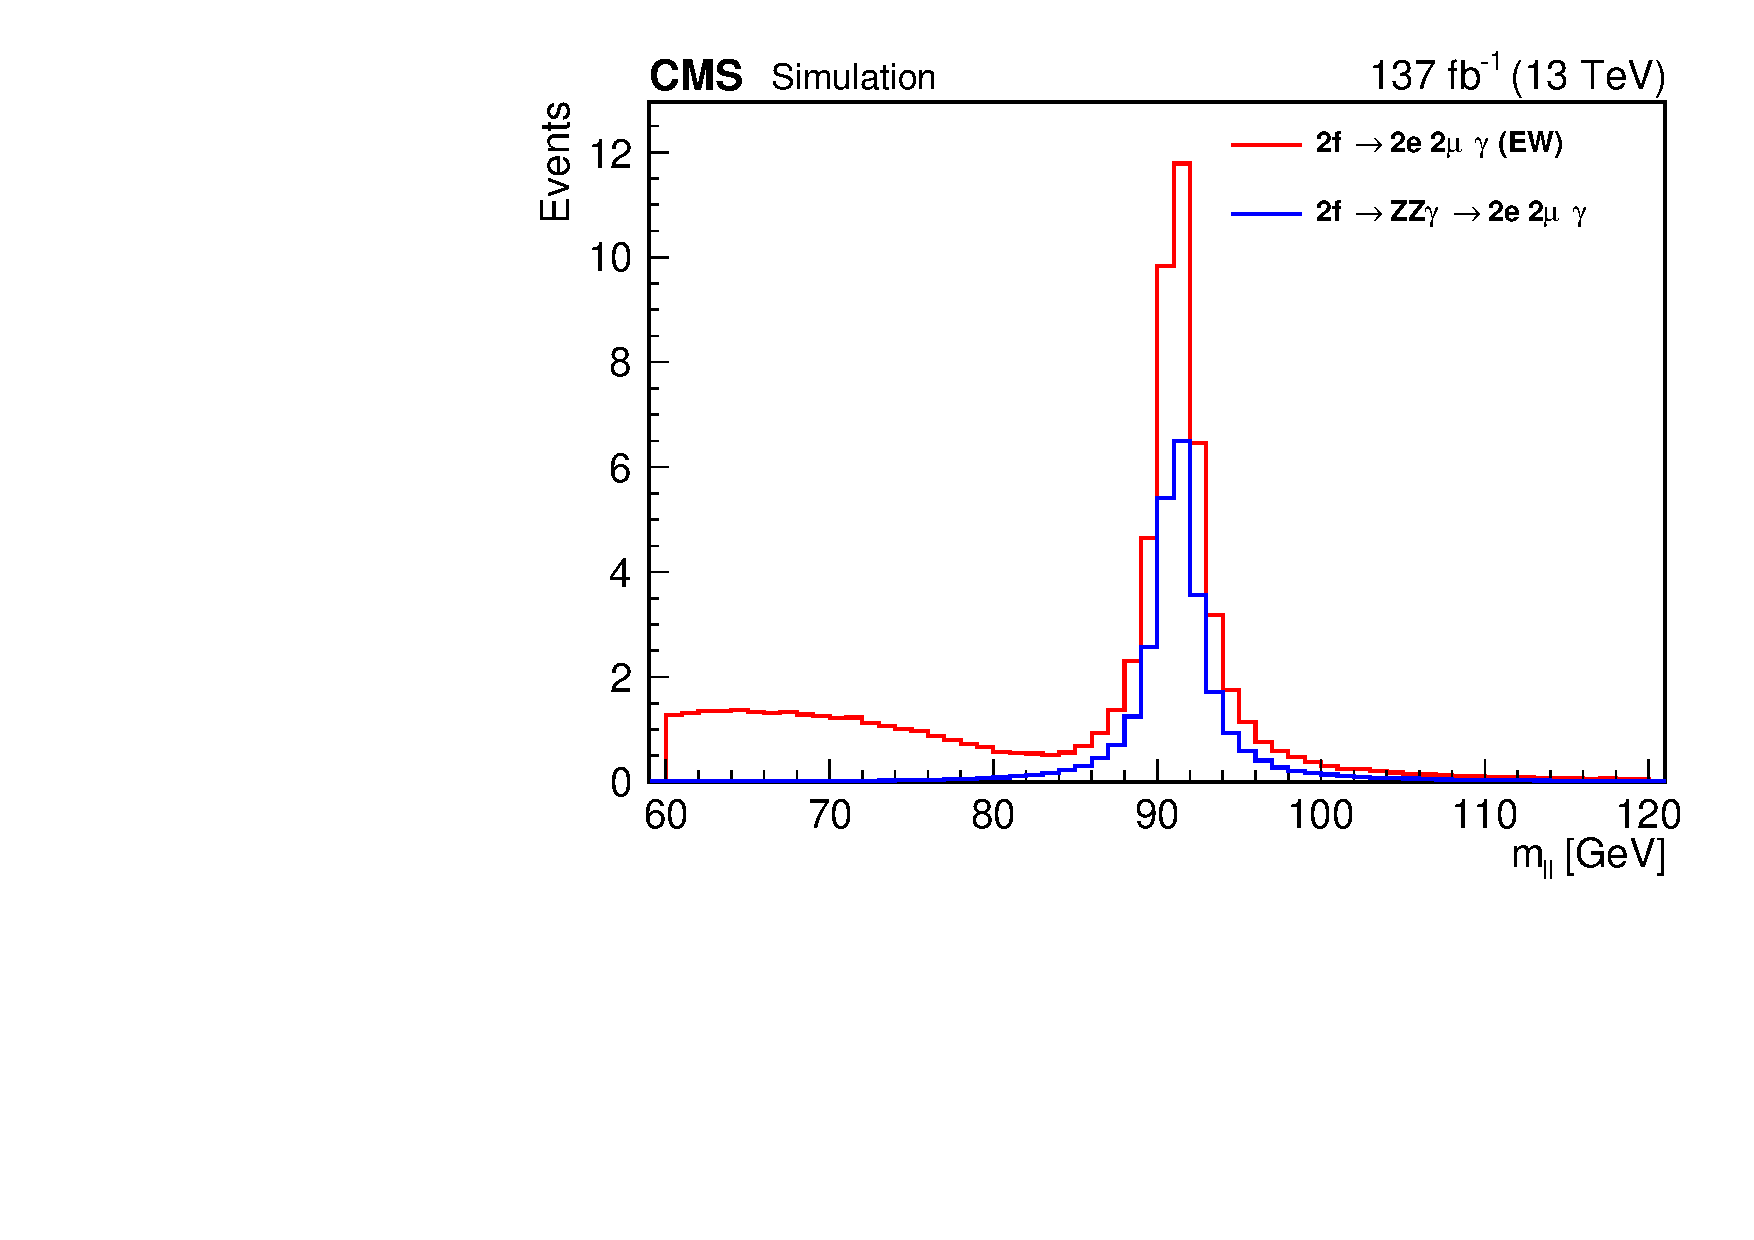
\includegraphics[width=.45\textwidth]{genstudy_mll.pdf}}\hfill
  \subfigure [$\pt^\PGg$]   {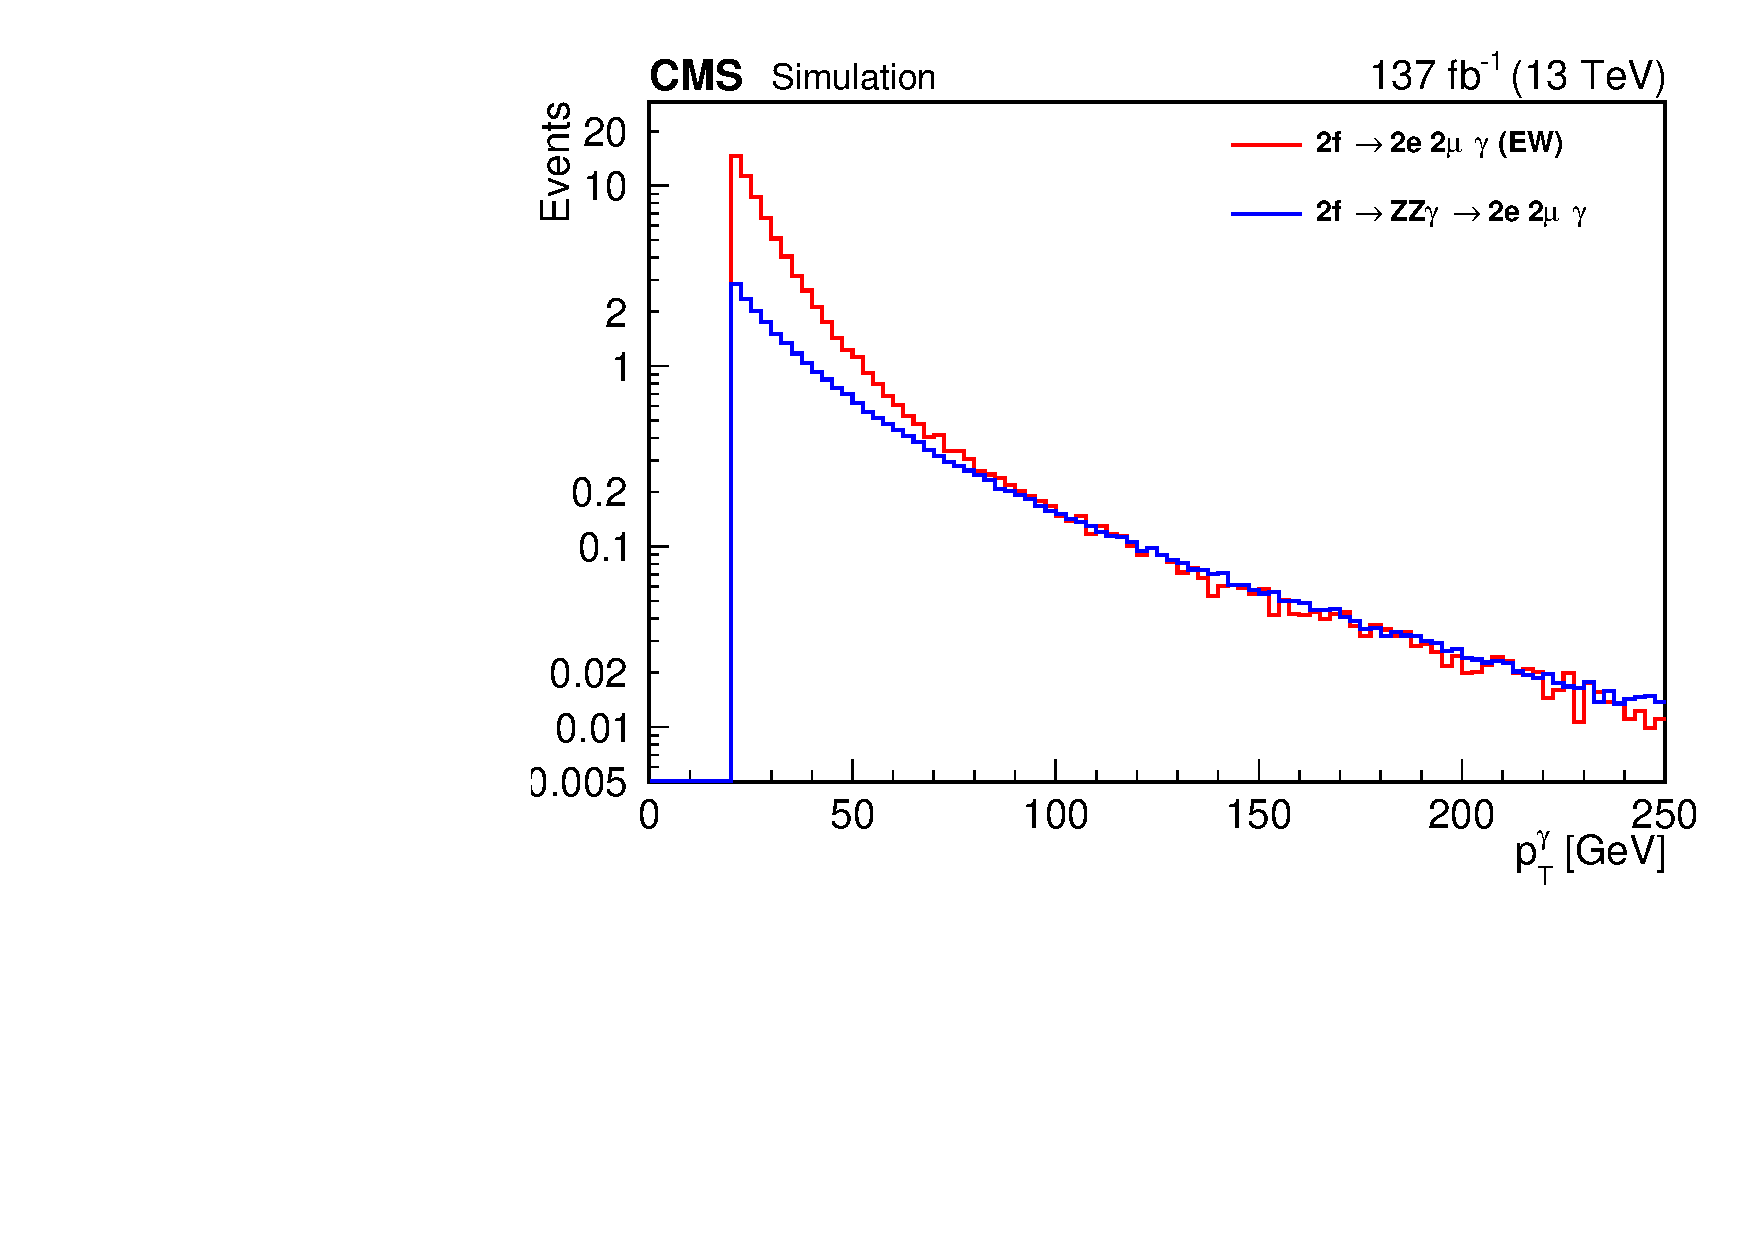
\includegraphics[width=.45\textwidth]{genstudy_ptGamma.pdf}}\hfill\mbox{}
  \caption{Invariant mass of the same-flavour opposite-sign lepton pairs and the transverse momentum of the photon
  in the two MC samples produced for the study of the fraction of FSR events in the $\Pp\Pp \to 4\Pl\PGg$ process.}
  \label{fig:genstudy}
\end{figure}
